\documentclass[12pt,a4paper]{article}

% ------------------------------------------------------------
% Packages
% ------------------------------------------------------------
\usepackage[margin=1in]{geometry}
\usepackage{amsmath,amssymb,bm}
\usepackage{graphicx}
\usepackage{float}
\usepackage{subcaption}
\usepackage{booktabs}
\usepackage{siunitx}
\usepackage{hyperref}
\usepackage{xcolor}
\usepackage{array}
\usepackage{indentfirst}
\usepackage{setspace}
\usepackage{enumitem}
\usepackage{titlesec}
\usepackage{caption}

% ------------------------------------------------------------
% Paragraph and spacing
% ------------------------------------------------------------
\setlength{\parindent}{2.7em}
\setlength{\parskip}{1.1\baselineskip}
\setstretch{1.25}

\setlist[itemize]{
    topsep=0.5em,
    itemsep=0.3em,
    parsep=0em,
    leftmargin=2.4em
}

\makeatletter
\let\@afterindentfalse\@afterindenttrue
\@afterindenttrue
\makeatother

\titlespacing*{\section}{0pt}{2.0em}{1.0em}
\titlespacing*{\subsection}{0pt}{1.6em}{0.8em}

\setlength{\abovecaptionskip}{0.5em}
\setlength{\belowcaptionskip}{0.7em}
\setlength{\textfloatsep}{1.2em}
\setlength{\floatsep}{1.2em}
\setlength{\intextsep}{1.2em}

\graphicspath{{part2_results/}{figures/}}

\hypersetup{
    colorlinks=true,
    linkcolor=blue,
    citecolor=blue,
    urlcolor=blue
}

% ------------------------------------------------------------
% Two-figure side-by-side helper
% ------------------------------------------------------------
\newcommand{\twolargefigs}[4]{%
\begin{figure}[htbp]
    \centering
    \begin{subfigure}{0.49\textwidth}
        \centering
        \includegraphics[width=\textwidth]{#1}
        \caption{$T=\SI{3}{s}$}
    \end{subfigure}
    \hfill
    \begin{subfigure}{0.49\textwidth}
        \centering
        \includegraphics[width=\textwidth]{#2}
        \caption{$T=\SI{6}{s}$}
    \end{subfigure}
    \caption{#3}
    \label{#4}
\end{figure}
}

% ------------------------------------------------------------
% Title
% ------------------------------------------------------------
\begin{document}

% ------------------------------------------------------------
% Title page
% ------------------------------------------------------------
\begin{titlepage}
    \centering
    \vspace*{0.4cm}
    \includegraphics[width=0.8\textwidth]{MSFEA_Logo_black.png}
    \vspace{1cm}

    {\Large\textbf{EECE 661 / MECH 641 Robotics}\par}
    {\large Professor Hussein Hussein\par}
    \vspace{0.6cm}

    {\Huge\textbf{Inverse Kinematics, Trajectory Control, and Torque Computation of the Dobot CR10 Robotic Manipulator}\par}
    \vspace{0.6cm}

    {\Large\textbf{by}\par}
    \vspace{0.45cm}
    {\large
    Khalil Al Wazzan\\
    Helene Jabbour\\
    Muche Workie\par}

    \vspace{0.4cm}
    {\large Spring 2025/2026\par}
\end{titlepage}

% ------------------------------------------------------------
% Abstract page
% ------------------------------------------------------------
\begin{titlepage}
    \centering
    \vspace*{\fill}

    {\Large\textbf{Abstract}\par}
    \vspace{1.0cm}

    \begin{minipage}{0.82\textwidth}
    \setlength{\parindent}{2.7em}
    \setlength{\parskip}{1.0em}
    \setstretch{1.25}

    This report presents a complete software pipeline for Cartesian trajectory generation,
    inverse kinematics, Jacobian-based differential kinematics, and joint torque computation
    for the Dobot CR10 robotic manipulator. The work addresses the following central question:
    given a desired end-effector trajectory, what joint torques are required for the robot
    to execute that motion?

    The pipeline begins from a desired Cartesian path and produces the corresponding joint
    position, velocity, acceleration, and actuator torque trajectories using the Pinocchio
    robotics library. Two end-effector paths are studied --- a straight-line trajectory and a
    circular trajectory parallel to the ground --- both generated using fifth-order polynomial
    time scaling. The complete pipeline is evaluated for two motion durations, \SI{3}{s} and
    \SI{6}{s}, which allows the effect of timing on the dynamic requirements to be analyzed
    independently of path geometry. The results show that doubling the duration approximately
    halves joint velocity peaks and reduces acceleration peaks by a factor of four, while
    torque components dominated by gravity remain large even for the slower motion.

    \end{minipage}

    \vspace*{\fill}
\end{titlepage}

\tableofcontents
\newpage

% ============================================================
\section{Introduction and Project Objective}
% ============================================================

The Dobot CR10 is a six-degree-of-freedom serial robotic manipulator used in research and
light industrial applications. Commanding such a robot along a desired Cartesian path is not
straightforward: the path must first be converted into joint-space coordinates through inverse
kinematics, and the resulting joint motion must be consistent with the physical equations of
motion if the actual actuator torques are to be computed correctly.

\begin{figure}[H]
    \centering
    \includegraphics[width=0.60\textwidth]{cr10.png}
    \caption{Dobot CR10 robotic manipulator used in this study.}
    \label{fig:dobot_cr10}
\end{figure}

The project addresses this problem in two phases. In the first phase, inverse kinematics was
implemented and used to command the CR10 in RViz through a custom ROS~2 node. This established
the geometric relationship between end-effector position and joint configuration. In the second
phase, the same trajectory framework was extended to a full dynamics pipeline: joint positions,
velocities, and accelerations were computed from a desired Cartesian path, and Pinocchio's
inverse dynamics solver was then used to compute the actuator torques required at every time
step.

The central question motivating the second phase is the following: given a desired end-effector
trajectory, what joint torques are required to move the Dobot CR10 along that trajectory? This
question is practically relevant because a trajectory that is kinematically reachable may impose
very different actuator requirements depending on how quickly it is executed. A faster motion
demands larger accelerations and therefore larger dynamic torques, while gravity torques persist
regardless of speed.

The full computational pipeline is described by
\begin{equation}
    \bm{x}_d(t),\ \dot{\bm{x}}_d(t),\ \ddot{\bm{x}}_d(t)
    \;\longrightarrow\;
    \bm{q}(t),\ \dot{\bm{q}}(t),\ \ddot{\bm{q}}(t)
    \;\longrightarrow\;
    \bm{\tau}(t),
    \label{eq:pipeline}
\end{equation}
where $\bm{x}_d(t)$ is the desired Cartesian trajectory, $\bm{q}(t)$ is the joint position
trajectory obtained through inverse kinematics, and $\bm{\tau}(t)$ is the required actuator
torque trajectory obtained through the Recursive Newton-Euler Algorithm (RNEA).

The specific objectives of the project are:
\begin{itemize}
    \item generate smooth Cartesian trajectories for straight-line and circular end-effector
          motions using fifth-order time scaling;
    \item compute the joint position trajectory $\bm{q}(t)$ using iterative inverse kinematics;
    \item compute the joint velocity trajectory $\dot{\bm{q}}(t)$ from the translational
          end-effector Jacobian;
    \item compute the joint acceleration trajectory $\ddot{\bm{q}}(t)$ using the Jacobian time
          derivative;
    \item derive the general equations of motion of the manipulator and apply Pinocchio inverse
          dynamics to obtain $\bm{\tau}(t)$;
    \item study and interpret the effect of motion duration on joint velocity, acceleration, and
          torque peaks.
\end{itemize}

% ============================================================
\section{Dobot CR10 Model}
% ============================================================

The robot model was loaded from the CR10 URDF file using Pinocchio. The resulting model has
\begin{equation}
    n_q = 6, \qquad n_v = 6,
\end{equation}
where $n_q$ is the configuration dimension and $n_v$ is the velocity dimension. Both are equal
to six because the robot has six revolute joints, each contributing one degree of freedom. The
joint order used throughout the implementation is
\begin{equation}
    \texttt{joint1},\ \texttt{joint2},\ \texttt{joint3},\
    \texttt{joint4},\ \texttt{joint5},\ \texttt{joint6}.
\end{equation}
All joint-space signals and numerical tables in this report follow this ordering. The
end-effector frame selected for Cartesian trajectory tracking is \texttt{Link6}, which
represents the distal frame whose position is controlled during both trajectory tasks.

A key implementation decision was to use Pinocchio as the exclusive source of robot
kinematics and dynamics. Earlier versions of the code maintained a parallel symbolic kinematic
model derived from Denavit-Hartenberg parameters, which was used inside the inverse kinematics
solver. The final implementation discards this dual-model approach and relies on Pinocchio for
all computations: forward kinematics, Jacobian evaluation, Jacobian time variation, and inverse
dynamics. Using a single consistent model eliminates the possibility of numerical mismatch
between the kinematics used in IK and the kinematics used in the Jacobian-based velocity and
acceleration computation. Such mismatches would corrupt the torque trajectory because the RNEA
solver would receive joint accelerations that are inconsistent with the robot geometry it
assumes.

% ============================================================
\section{Trajectory Generation}
% ============================================================

Two end-effector trajectories were studied. A straight-line trajectory tests whether the robot
can follow a simple Cartesian segment without deviation. A circular trajectory parallel to the
ground is more demanding because the direction of motion changes continuously throughout the
motion, which requires greater joint coordination and produces stronger centripetal acceleration
terms.

Both trajectories were parameterized using fifth-order polynomial time scaling. Time scaling
separates path geometry from motion timing: the path specifies where the end effector moves,
while the time-scaling function determines the velocity profile along that path. The same
geometric path can therefore be studied under different timing conditions without changing
the IK solution sequence.

\subsection{Quintic Time Scaling}

For a motion of total duration $T$, the time-scaling variable is defined as
\begin{equation}
    s(t) = 10\!\left(\frac{t}{T}\right)^{\!3}
           - 15\!\left(\frac{t}{T}\right)^{\!4}
           + 6\!\left(\frac{t}{T}\right)^{\!5}.
    \label{eq:quintic}
\end{equation}
This polynomial satisfies the boundary conditions
\begin{equation}
    s(0) = 0, \qquad s(T) = 1,
\end{equation}
and additionally enforces zero velocity and zero acceleration at both endpoints:
\begin{equation}
    \dot{s}(0) = \dot{s}(T) = 0, \qquad
    \ddot{s}(0) = \ddot{s}(T) = 0.
\end{equation}
The zero-velocity boundary condition ensures that the end effector starts and ends at rest.
The zero-acceleration boundary condition ensures that no impulsive torque is required at the
trajectory endpoints --- a property that is later verified numerically through the RNEA
boundary check described in Section~\ref{sec:rnea}.

The time derivatives of $s(t)$ are needed because the dynamics pipeline requires Cartesian
velocities and accelerations. Applying the chain rule gives
\begin{equation}
    \dot{s}(t) = \frac{1}{T}\!\left[
        30\!\left(\frac{t}{T}\right)^{\!2}
      - 60\!\left(\frac{t}{T}\right)^{\!3}
      + 30\!\left(\frac{t}{T}\right)^{\!4}
    \right],
\end{equation}
\begin{equation}
    \ddot{s}(t) = \frac{1}{T^2}\!\left[
        60\!\left(\frac{t}{T}\right)
      - 180\!\left(\frac{t}{T}\right)^{\!2}
      + 120\!\left(\frac{t}{T}\right)^{\!3}
    \right].
\end{equation}
The $1/T$ and $1/T^2$ prefactors mean that halving the duration approximately doubles the
velocity profile and quadruples the acceleration profile, which explains the duration effects
observed in the results.

Both trajectories were evaluated for
\begin{equation}
    T \in \{3,\,6\}\ \si{s}, \qquad \Delta t = \SI{0.01}{s}.
\end{equation}

\subsection{Straight-Line Trajectory}

The straight-line trajectory moves the end effector between two Cartesian points
\begin{equation}
    \bm{x}_A =
    \begin{bmatrix} 0.45 \\ -0.30 \\ 0.45 \end{bmatrix}\si{m},
    \qquad
    \bm{x}_B =
    \begin{bmatrix} 0.45 \\ 0.30 \\ 0.45 \end{bmatrix}\si{m}.
\end{equation}
The desired Cartesian position, velocity, and acceleration at each time step are
\begin{align}
    \bm{x}_d(t)      &= \bm{x}_A + s(t)\,(\bm{x}_B - \bm{x}_A), \\
    \dot{\bm{x}}_d(t)  &= \dot{s}(t)\,(\bm{x}_B - \bm{x}_A), \\
    \ddot{\bm{x}}_d(t) &= \ddot{s}(t)\,(\bm{x}_B - \bm{x}_A).
\end{align}
In this trajectory the $x$ and $z$ coordinates are constant, while the $y$ coordinate sweeps
from \SI{-0.30}{m} to \SI{+0.30}{m}. The XY path projection should therefore appear as a
straight vertical line, which provides a simple geometric check on the trajectory generation
and IK tracking.

\subsection{Circular Trajectory Parallel to the Ground}

The circular trajectory maintains constant height while the end effector traces a full circle
in the horizontal plane. The selected center and radius are
\begin{equation}
    \bm{x}_c =
    \begin{bmatrix} 0.50 \\ 0.00 \\ 0.45 \end{bmatrix}\si{m},
    \qquad R = \SI{0.12}{m}.
\end{equation}
The angular position along the circle is linked to the time-scaling variable by
\begin{equation}
    \theta(t) = 2\pi\,s(t), \qquad
    \dot{\theta}(t) = 2\pi\,\dot{s}(t), \qquad
    \ddot{\theta}(t) = 2\pi\,\ddot{s}(t).
\end{equation}
The Cartesian trajectory components are
\begin{align}
    x_d(t) &= x_c + R\cos\!\bigl(\theta(t)\bigr), \\
    y_d(t) &= y_c + R\sin\!\bigl(\theta(t)\bigr), \\
    z_d(t) &= z_c.
\end{align}
Differentiating with respect to time gives the velocity components
\begin{align}
    \dot{x}_d(t) &= -R\sin\!\bigl(\theta(t)\bigr)\,\dot{\theta}(t), \\
    \dot{y}_d(t) &=  R\cos\!\bigl(\theta(t)\bigr)\,\dot{\theta}(t), \\
    \dot{z}_d(t) &= 0,
\end{align}
and the acceleration components
\begin{align}
    \ddot{x}_d(t) &= -R\cos\!\bigl(\theta(t)\bigr)\,\dot{\theta}^2(t)
                     - R\sin\!\bigl(\theta(t)\bigr)\,\ddot{\theta}(t), \\
    \ddot{y}_d(t) &= -R\sin\!\bigl(\theta(t)\bigr)\,\dot{\theta}^2(t)
                     + R\cos\!\bigl(\theta(t)\bigr)\,\ddot{\theta}(t), \\
    \ddot{z}_d(t) &= 0.
\end{align}
The acceleration expressions contain two terms each: a centripetal term proportional to
$\dot{\theta}^2$ and a tangential term proportional to $\ddot{\theta}$. Both are present even
when the speed profile is smooth, because the direction of the velocity vector rotates
continuously around the circle. This makes the circular trajectory more demanding than the
straight-line case in terms of joint accelerations and, consequently, actuator torques.

% ============================================================
\section{Inverse Kinematics}
% ============================================================

For each desired Cartesian position $\bm{x}_d(t_k)$, inverse kinematics was used to compute
the joint configuration $\bm{q}(t_k)$ that places the end-effector frame \texttt{Link6} at
the target. The output of this stage is the joint position sequence
\begin{equation}
    \bm{q}(t_0),\;\bm{q}(t_1),\;\ldots,\;\bm{q}(t_N),
\end{equation}
which serves as the input to the Jacobian-based velocity and acceleration computation in
Part~B.

The solver is iterative and based on damped least-squares (DLS), but the primary task is
\emph{position-only}: at each iteration, Pinocchio computes the current end-effector position
and the translational Jacobian $J_p \in \mathbb{R}^{3\times 6}$, and the primary joint update
is obtained from the DLS pseudoinverse of $J_p$ (IK damping set to $10^{-2}$). This matches the
project objective, where the Cartesian trajectory is specified for position and not for a
prescribed orientation.

Because the CR10 has six joints and the task has three constraints, the IK is redundant. The
remaining nullspace freedom is resolved with secondary objectives projected through
$N = I - J_p^\dagger J_p$: continuity toward the previous solution, mild joint-centering, and
a soft joint-6 anchor. The joint-6 reference is fixed to the first accepted waypoint and reused
for the full trajectory. The wrist term uses a \emph{linear} (non-wrapped) error
$(q_{6,\mathrm{ref}}-q_6)$, which penalizes $2\pi$-equivalent drift and prevents winding
accumulation on closed paths.
If the translational Jacobian rank drops below three while the position error is still large,
that candidate is rejected as near-singular.

For the first trajectory waypoint, a multi-seed exhaustive search selects the best solution
from a set of canonical seed configurations. For subsequent waypoints, a fast single-seed
solve starting from the previous joint configuration is attempted first. If this fails the
tolerance or does not converge, a shorter candidate search is performed as a fallback. This
warm-start strategy promotes joint-space continuity along the trajectory.

All accepted IK solutions are validated against a position tolerance of \SI{5}{mm}. Any
solution with a larger end-effector position error is rejected, which prevents inaccurate
configurations from propagating through the Jacobian and dynamics computations.

% ============================================================
\section{Jacobian-Based Velocity and Acceleration}
% ============================================================

Once the joint position trajectory is known, the joint velocities and accelerations are
computed using the end-effector Jacobian and its time derivative. Numerical differentiation
of the joint positions was deliberately not used, because it would amplify quantization noise
and would not make use of the differential kinematics structure of the robot.

\subsection{Joint Velocity}

The relationship between the Cartesian end-effector velocity and the joint velocity is
\begin{equation}
    \dot{\bm{x}}_d = J_p(\bm{q})\,\dot{\bm{q}},
    \label{eq:vel_fwd}
\end{equation}
where $J_p(\bm{q}) \in \mathbb{R}^{3 \times 6}$ is the translational part of the end-effector
Jacobian. Since the Jacobian is not square, the joint velocity cannot be obtained by direct
inversion. The damped least-squares pseudoinverse is used instead:
\begin{equation}
    \dot{\bm{q}}(t_k)
    = J_p^{\,T}\!\left(J_p J_p^{\,T} + \lambda^2 I\right)^{-1}\dot{\bm{x}}_d(t_k),
    \label{eq:qdot}
\end{equation}
with damping factor $\lambda = 10^{-3}$. This value was chosen to provide sufficient
regularization near singular or near-singular configurations without appreciably reducing
tracking accuracy in the interior of the workspace. A much smaller value such as $10^{-6}$
can produce arbitrarily large joint velocities when the Jacobian loses rank.

The Jacobian is computed by Pinocchio using the \texttt{LOCAL\_WORLD\_ALIGNED} reference frame,
which expresses translational velocities in the world frame. The same reference frame is used
consistently for all Jacobian and Jacobian time derivative computations.

\subsection{Joint Acceleration}

Differentiating~\eqref{eq:vel_fwd} with respect to time gives
\begin{equation}
    \ddot{\bm{x}}_d = J_p(\bm{q})\,\ddot{\bm{q}}
                    + \dot{J}_p(\bm{q},\dot{\bm{q}})\,\dot{\bm{q}}.
    \label{eq:acc_fwd}
\end{equation}
Rearranging for the unknown $\ddot{\bm{q}}$ yields
\begin{equation}
    J_p(\bm{q})\,\ddot{\bm{q}} = \ddot{\bm{x}}_d - \dot{J}_p(\bm{q},\dot{\bm{q}})\,\dot{\bm{q}},
\end{equation}
and solving with the same damped pseudoinverse gives
\begin{equation}
    \ddot{\bm{q}}(t_k)
    = J_p^{\,T}\!\left(J_p J_p^{\,T} + \lambda^2 I\right)^{-1}
      \!\left[\ddot{\bm{x}}_d(t_k) - \dot{J}_p(t_k)\,\dot{\bm{q}}(t_k)\right].
    \label{eq:qddot}
\end{equation}
The term $\dot{J}_p\,\dot{\bm{q}}$ accounts for the rate of change of the Jacobian due to
joint motion. Omitting this term is equivalent to assuming a frozen Jacobian, which introduces
an error in the acceleration computation that grows with joint velocity. The Jacobian time
derivative is evaluated using Pinocchio's \texttt{computeJointJacobiansTimeVariation} and
\texttt{getFrameJacobianTimeVariation} functions, called after
\texttt{forwardKinematics($\bm{q}_k$, $\dot{\bm{q}}_k$)} to ensure the internal data
structures reflect both the current position and velocity.

The velocity and acceleration are computed in a single pass per time step: $\dot{\bm{q}}_k$
is determined first from~\eqref{eq:qdot}, and $\ddot{\bm{q}}_k$ is then determined from
\eqref{eq:qddot} using the $\dot{\bm{q}}_k$ just computed. This avoids the inconsistency
that would arise from computing the full velocity trajectory in a separate loop before
computing accelerations, since the Jacobian time derivative in the second computation must
correspond to the same configuration and velocity used for the first.

% ============================================================
\section{Robot Dynamics and Torque Computation}
% ============================================================

\subsection{Equations of Motion}
\label{sec:eom}

The joint-space equation of motion for an $n$-DOF rigid-body manipulator is
\begin{equation}
    M(\bm{q})\,\ddot{\bm{q}}
    + C(\bm{q},\dot{\bm{q}})\,\dot{\bm{q}}
    + \bm{g}(\bm{q}) = \bm{\tau}.
    \label{eq:eom}
\end{equation}
Rearranged for the required actuator torque:
\begin{equation}
    \bm{\tau} = M(\bm{q})\,\ddot{\bm{q}}
              + C(\bm{q},\dot{\bm{q}})\,\dot{\bm{q}}
              + \bm{g}(\bm{q}).
    \label{eq:tau}
\end{equation}

The matrix $M(\bm{q}) \in \mathbb{R}^{n \times n}$ is the joint-space inertia matrix. It
encodes the resistance of the robot to joint acceleration. Because the robot's link inertia
tensors are fixed in body frames, $M(\bm{q})$ changes as the configuration changes: a fully
extended arm presents a larger effective inertia to the base joint than a compact configuration.

The term $C(\bm{q},\dot{\bm{q}})\,\dot{\bm{q}} \in \mathbb{R}^{n}$ collects the Coriolis and
centrifugal torques. These arise from the cross-coupling between joint velocities: when one
joint rotates, the angular momentum of the links distal to that joint changes, which induces
reaction torques on other joints. These terms are proportional to products of joint velocities
and are therefore negligible at low speeds but can be significant for the faster,
shorter-duration trajectories.

The vector $\bm{g}(\bm{q}) \in \mathbb{R}^{n}$ is the gravity torque vector. It represents
the torque each actuator must exert to keep the robot stationary against gravity at the current
configuration. This term does not vanish when the robot moves slowly. As a result, joints that
carry the main arm structure --- joints 2 and 3 in the CR10 --- can require large torques even
when the trajectory is very slow.

\subsection{Torque Computation via Pinocchio RNEA}
\label{sec:rnea}

Given the joint trajectories $\bm{q}(t)$, $\dot{\bm{q}}(t)$, $\ddot{\bm{q}}(t)$, the
torque at each time step is computed using the Recursive Newton-Euler Algorithm:
\begin{equation}
    \bm{\tau}(t_k)
    = \mathrm{RNEA}\!\left(\bm{q}(t_k),\,\dot{\bm{q}}(t_k),\,\ddot{\bm{q}}(t_k)\right).
    \label{eq:rnea}
\end{equation}
The RNEA evaluates equation~\eqref{eq:tau} efficiently without forming $M$, $C$, or
$\bm{g}$ explicitly. For the six-joint CR10 model the output torque vector is
\begin{equation}
    \bm{\tau}(t_k) =
    \begin{bmatrix}
        \tau_1(t_k) & \tau_2(t_k) & \tau_3(t_k) &
        \tau_4(t_k) & \tau_5(t_k) & \tau_6(t_k)
    \end{bmatrix}^{\!T}.
\end{equation}

A boundary consistency check is applied after the torque computation. The quintic time scaling
guarantees $\dot{\bm{q}}(0) = \dot{\bm{q}}(T) = \bm{0}$ and
$\ddot{\bm{q}}(0) = \ddot{\bm{q}}(T) = \bm{0}$. Substituting into~\eqref{eq:tau}:
\begin{equation}
    \dot{\bm{q}} = \bm{0},\quad \ddot{\bm{q}} = \bm{0}
    \;\Rightarrow\;
    \bm{\tau} = \bm{g}(\bm{q}).
    \label{eq:gravity_check}
\end{equation}
The implementation verifies this by calling the RNEA with zero velocity and acceleration at
$t_0$ and $t_N$ and comparing the result to the computed $\bm{\tau}(t_0)$ and $\bm{\tau}(t_N)$.
Any significant discrepancy indicates an inconsistency in the IK solution or the Pinocchio
model and is reported as a warning.

% ============================================================
\section{Results}
% ============================================================

This section presents the numerical results for both trajectories and both motion durations.
For each case, the required plots are: Cartesian path, joint positions, joint velocities,
joint accelerations, and joint torques. The joint most relevant for dynamic analysis is
discussed in each subsection, and per-joint peak values are tabulated at the end of each
trajectory discussion.

\subsection{Straight-Line Trajectory}

Figure~\ref{fig:straight_cartesian} shows the Cartesian trajectory for the straight-line case.
The $x$ and $z$ coordinates are constant throughout, and the $y$ coordinate moves smoothly
from \SI{-0.30}{m} to \SI{+0.30}{m}. The XY path projection confirms a straight vertical
line with no lateral deviation, which validates both the trajectory generator and the IK
tracking. The two durations produce the same geometric path and differ only in timing.

\twolargefigs
{straight_T3p0s_cartesian.png}
{straight_T6p0s_cartesian.png}
{Cartesian straight-line trajectory: position components (left panel) and XY path projection (right panel).}
{fig:straight_cartesian}

Figure~\ref{fig:straight_q} shows the joint positions. The profiles are nearly identical for
both durations, which is expected: the same Cartesian path leads to nearly the same IK branch,
and changing $T$ mainly affects timing-dependent quantities. The largest excursion is in joint~1
(base rotation), while joints~4--5 adapt smoothly to keep the end effector on the line.
Joint~6 remains tightly bounded (about \SIrange{-0.0102}{-0.0077}{rad}), confirming that the
fixed-anchor nullspace term suppresses wrist winding.

\twolargefigs
{straight_T3p0s_q.png}
{straight_T6p0s_q.png}
{Joint positions for the straight-line trajectory.}
{fig:straight_q}

Figure~\ref{fig:straight_qdot} shows the joint velocities. The $T=\SI{3}{s}$ peaks are
approximately twice those of $T=\SI{6}{s}$, consistent with the $1/T$ scaling of the quintic
derivative. Joint~1 dominates the velocity profile (\SI{0.8442}{rad/s} at $T=\SI{3}{s}$)
because the lateral $y$-direction sweep maps primarily onto base-joint rotation, while
joint~6 remains essentially zero.

\twolargefigs
{straight_T3p0s_qdot.png}
{straight_T6p0s_qdot.png}
{Joint velocities for the straight-line trajectory.}
{fig:straight_qdot}

Figure~\ref{fig:straight_qddot} shows the joint accelerations. The $T=\SI{3}{s}$ peaks are
roughly four times those of $T=\SI{6}{s}$, consistent with $1/T^2$ scaling. All profiles
start and end at zero, confirming the quintic boundary conditions. This zero-acceleration
boundary is what allows the RNEA boundary check~\eqref{eq:gravity_check} to hold: without
it, a non-zero initial acceleration would require a non-zero dynamic torque component at
$t=0$, which would violate the gravity-only prediction.

\twolargefigs
{straight_T3p0s_qddot.png}
{straight_T6p0s_qddot.png}
{Joint accelerations for the straight-line trajectory.}
{fig:straight_qddot}

Figure~\ref{fig:straight_tau} shows the torque trajectories. Joint~2 carries the largest
torque, reaching approximately \SI{65.06}{N.m} at $T=\SI{3}{s}$ and \SI{64.84}{N.m} at
$T=\SI{6}{s}$. This weak duration dependence indicates gravity-dominated loading at the
shoulder. Joint~1 shows a strong duration effect, dropping from \SI{2.98}{N.m} to
\SI{0.75}{N.m}, while joint~3 decreases more modestly from \SI{3.91}{N.m} to \SI{3.55}{N.m}.
Joints~4--6 remain comparatively small.

\twolargefigs
{straight_T3p0s_tau.png}
{straight_T6p0s_tau.png}
{Joint torques for the straight-line trajectory.}
{fig:straight_tau}

\begin{table}[H]
\centering
\caption{Straight-line trajectory: per-joint peak values for both durations.}
\label{tab:straight_peaks}
\resizebox{\textwidth}{!}{%
\begin{tabular}{lcccccc}
\toprule
Quantity & joint1 & joint2 & joint3 & joint4 & joint5 & joint6 \\
\midrule
$\max|\dot{q}|$ at $T=\SI{3}{s}$ [rad/s]   & 0.8442 & 0.0799 & 0.2018 & 0.0185 & 0.1775 & 0.0000 \\
$\max|\dot{q}|$ at $T=\SI{6}{s}$ [rad/s]   & 0.4222 & 0.0402 & 0.1009 & 0.0093 & 0.0887 & 0.0000 \\
$\max|\ddot{q}|$ at $T=\SI{3}{s}$ [rad/s$^2$] & 0.9521 & 0.2839 & 0.5237 & 0.0420 & 0.2387 & 0.0000 \\
$\max|\ddot{q}|$ at $T=\SI{6}{s}$ [rad/s$^2$] & 0.2376 & 0.0711 & 0.1310 & 0.0104 & 0.0596 & 0.0000 \\
$\max|\tau|$ at $T=\SI{3}{s}$ [N$\cdot$m]  & 2.9820 & 65.0649 & 3.9149 & 1.3998 & 0.0037 & 0.00014 \\
$\max|\tau|$ at $T=\SI{6}{s}$ [N$\cdot$m]  & 0.7486 & 64.8403 & 3.5541 & 1.3979 & 0.0020 & 0.00005 \\
\bottomrule
\end{tabular}}
\end{table}

\subsection{Circular Trajectory}

Figure~\ref{fig:circle_cartesian} shows the circular trajectory. The XY projection confirms a
closed circle with radius \SI{0.12}{m} centered at $(0.50,\,0.00)$\,m, and the $z$ coordinate
remains constant at \SI{0.45}{m} throughout, confirming that the trajectory is parallel to the
ground. Both durations trace the same circle.

\twolargefigs
{circle_T3p0s_cartesian.png}
{circle_T6p0s_cartesian.png}
{Cartesian circular trajectory: position components and XY path projection.}
{fig:circle_cartesian}

Figure~\ref{fig:circle_q} shows the joint positions for the circular trajectory. More joints
participate visibly compared to the straight-line case, because maintaining a closed circular
path in the $xy$ plane requires coordinated motion in both directions simultaneously. All
profiles are smooth, indicating that the IK solver found a continuous solution branch
throughout the full circle. Joint~6 again stays nearly constant
(\SIrange{-0.0102}{-0.0077}{rad}), showing that the fixed-anchor nullspace regularization
remains effective on a closed path.

\twolargefigs
{circle_T3p0s_q.png}
{circle_T6p0s_q.png}
{Joint positions for the circular trajectory.}
{fig:circle_q}

Figure~\ref{fig:circle_qdot} shows the joint velocities. The circular trajectory produces
larger peaks than the straight-line case: the global peak for $T=\SI{3}{s}$ reaches
approximately \SI{1.49}{rad/s}, compared to \SI{0.84}{rad/s} for the line. Several joints
exhibit sign reversals during the motion because the required joint direction changes as the
end effector progresses around the circle. The $1/T$ ratio between the two durations is again
clearly visible.

\twolargefigs
{circle_T3p0s_qdot.png}
{circle_T6p0s_qdot.png}
{Joint velocities for the circular trajectory.}
{fig:circle_qdot}

Figure~\ref{fig:circle_qddot} shows the joint accelerations. The values are significantly
larger than for the straight-line trajectory: for $T=\SI{3}{s}$, the global peak reaches
approximately \SI{6.94}{rad/s^2} (joint~1), compared to \SI{0.95}{rad/s^2} for the
straight-line case. This difference reflects the centripetal acceleration inherent in circular
motion. At $T=\SI{6}{s}$, the global peak falls to approximately \SI{1.73}{rad/s^2},
consistent with the expected factor-of-four reduction from $1/T^2$ scaling.

\twolargefigs
{circle_T3p0s_qddot.png}
{circle_T6p0s_qddot.png}
{Joint accelerations for the circular trajectory.}
{fig:circle_qddot}

Figure~\ref{fig:circle_tau} shows the torque trajectories for the circular motion. Joints 2
and 1 show the strongest dynamic dependence. Joint~2 is globally dominant in both durations,
reaching approximately \SI{68.38}{N.m} at $T=\SI{3}{s}$ and \SI{67.90}{N.m} at $T=\SI{6}{s}$,
which indicates a large gravity baseline. Joint~1 drops from approximately \SI{19.02}{N.m}
to \SI{4.76}{N.m}, and joint~3 drops from \SI{13.04}{N.m} to \SI{9.84}{N.m}, confirming that
their peaks contain stronger inertial components than joint~2.

\twolargefigs
{circle_T3p0s_tau.png}
{circle_T6p0s_tau.png}
{Joint torques for the circular trajectory.}
{fig:circle_tau}

\begin{table}[H]
\centering
\caption{Circular trajectory: per-joint peak values for both durations.}
\label{tab:circle_peaks}
\resizebox{\textwidth}{!}{%
\begin{tabular}{lcccccc}
\toprule
Quantity & joint1 & joint2 & joint3 & joint4 & joint5 & joint6 \\
\midrule
$\max|\dot{q}|$ at $T=\SI{3}{s}$ [rad/s]      & 1.4856 & 0.4713 & 0.7212 & 0.1020 & 0.4331 & 0.0000 \\
$\max|\dot{q}|$ at $T=\SI{6}{s}$ [rad/s]      & 0.7423 & 0.2350 & 0.3614 & 0.0514 & 0.2168 & 0.0000 \\
$\max|\ddot{q}|$ at $T=\SI{3}{s}$ [rad/s$^2$] & 6.9352 & 4.2610 & 3.9437 & 1.1179 & 2.5555 & 0.0000 \\
$\max|\ddot{q}|$ at $T=\SI{6}{s}$ [rad/s$^2$] & 1.7335 & 1.0699 & 0.9879 & 0.2846 & 0.6381 & 0.0000 \\
$\max|\tau|$ at $T=\SI{3}{s}$ [N$\cdot$m]     & 19.0163 & 68.3778 & 13.0365 & 1.6598 & 0.0103 & 0.00103 \\
$\max|\tau|$ at $T=\SI{6}{s}$ [N$\cdot$m]     & 4.7581 & 67.9016 & 9.8436 & 1.5747 & 0.0038 & 0.00023 \\
\bottomrule
\end{tabular}}
\end{table}

% ============================================================
\section{Effect of Motion Duration}
% ============================================================

The duration study isolates the effect of timing from path geometry by running the full
pipeline twice on each trajectory: once at $T=\SI{3}{s}$ and once at $T=\SI{6}{s}$. The
geometric path is unchanged and the IK follows the same continuous branch in both runs; only
$\dot{s}$ and $\ddot{s}$ change, which propagates through to the Cartesian velocities,
accelerations, and finally the dynamic torque contributions.

\begin{table}[H]
\centering
\caption{Global peak values for the duration study.}
\label{tab:duration_summary}
\resizebox{\textwidth}{!}{%
\begin{tabular}{llccc}
\toprule
Trajectory & Duration &
$\max|\dot{q}|$ [rad/s] &
$\max|\ddot{q}|$ [rad/s$^2$] &
$\max|\tau|$ [N$\cdot$m] \\
\midrule
Straight & \SI{3}{s} & 0.8442 & 0.9521 & 65.0649 \\
Straight & \SI{6}{s} & 0.4222 & 0.2376 & 64.8403 \\
Circle   & \SI{3}{s} & 1.4856 & 6.9352 & 68.3778 \\
Circle   & \SI{6}{s} & 0.7423 & 1.7335 & 67.9016 \\
\bottomrule
\end{tabular}}
\end{table}

\paragraph{Effect on joint velocities.}
For both trajectories, doubling $T$ halves the global velocity peak. The straight-line peak
drops from \SI{0.8442}{rad/s} to \SI{0.4222}{rad/s} (ratio 2.00), and the circular peak
drops from \SI{1.4856}{rad/s} to \SI{0.7423}{rad/s} (ratio 2.00). This exact factor of two
follows directly from the $1/T$ derivative scaling of the quintic function and confirms that
the trajectory generation and IK pipeline behave as expected.

\paragraph{Effect on joint accelerations.}
The acceleration reduction is stronger. Doubling $T$ reduces acceleration peaks by
approximately a factor of four ($1/T^2$ scaling). For the straight-line trajectory the global
peak drops from \SI{0.9521}{rad/s^2} to \SI{0.2376}{rad/s^2} (ratio 4.01). For the circular
trajectory it drops from \SI{6.9352}{rad/s^2} to \SI{1.7335}{rad/s^2} (ratio 4.00). The
larger absolute values for the circular case reflect the centripetal term, which is absent in
the straight-line motion.

\paragraph{Effect on maximum torque.}
The torque response is more nuanced because actuator torques include both dynamic and static
contributions. For the straight-line trajectory, the global torque peak barely changes:
\SI{65.06}{N.m} versus \SI{64.84}{N.m}. This near-constant value reflects the dominance of
joint 2 gravity loading. The gravitational torque required to hold the main arm links in
place does not depend on how quickly the end effector moves. For the circular trajectory, the
global torque peak drops from \SI{68.38}{N.m} to \SI{67.90}{N.m}, a modest reduction that
again reflects the mix of gravity and dynamic loading, with joint 2 setting the envelope.

\paragraph{Effect on torque curve shape.}
The general shape of the torque profiles is preserved between durations: the same joints
dominate, and the torque curves exhibit the same qualitative features at corresponding
fractions of the trajectory. The slower trajectory reduces the amplitude of dynamic peaks and
softens sharp transitions, but the gravity-driven baseline remains at approximately the same
level. This is visible in Figures~\ref{fig:straight_duration_comparison} and
\ref{fig:circle_duration_comparison}.

\paragraph{Most affected joints.}
The joints whose torques change most significantly with duration are the joints with a large
dynamic contribution relative to their total load. For the straight-line trajectory, joint 1
shows the largest absolute change (about \SI{2.23}{N.m}), followed by joints 3
(\SI{0.36}{N.m}) and 2 (\SI{0.22}{N.m}). For the circular trajectory, the largest change is in
joint~1 (about \SI{14.26}{N.m}), followed by joint~3 (\SI{3.19}{N.m}) and joint~2
(\SI{0.48}{N.m}). Joints 4, 5, and 6 are much less affected in both cases.

\begin{figure}[H]
    \centering
    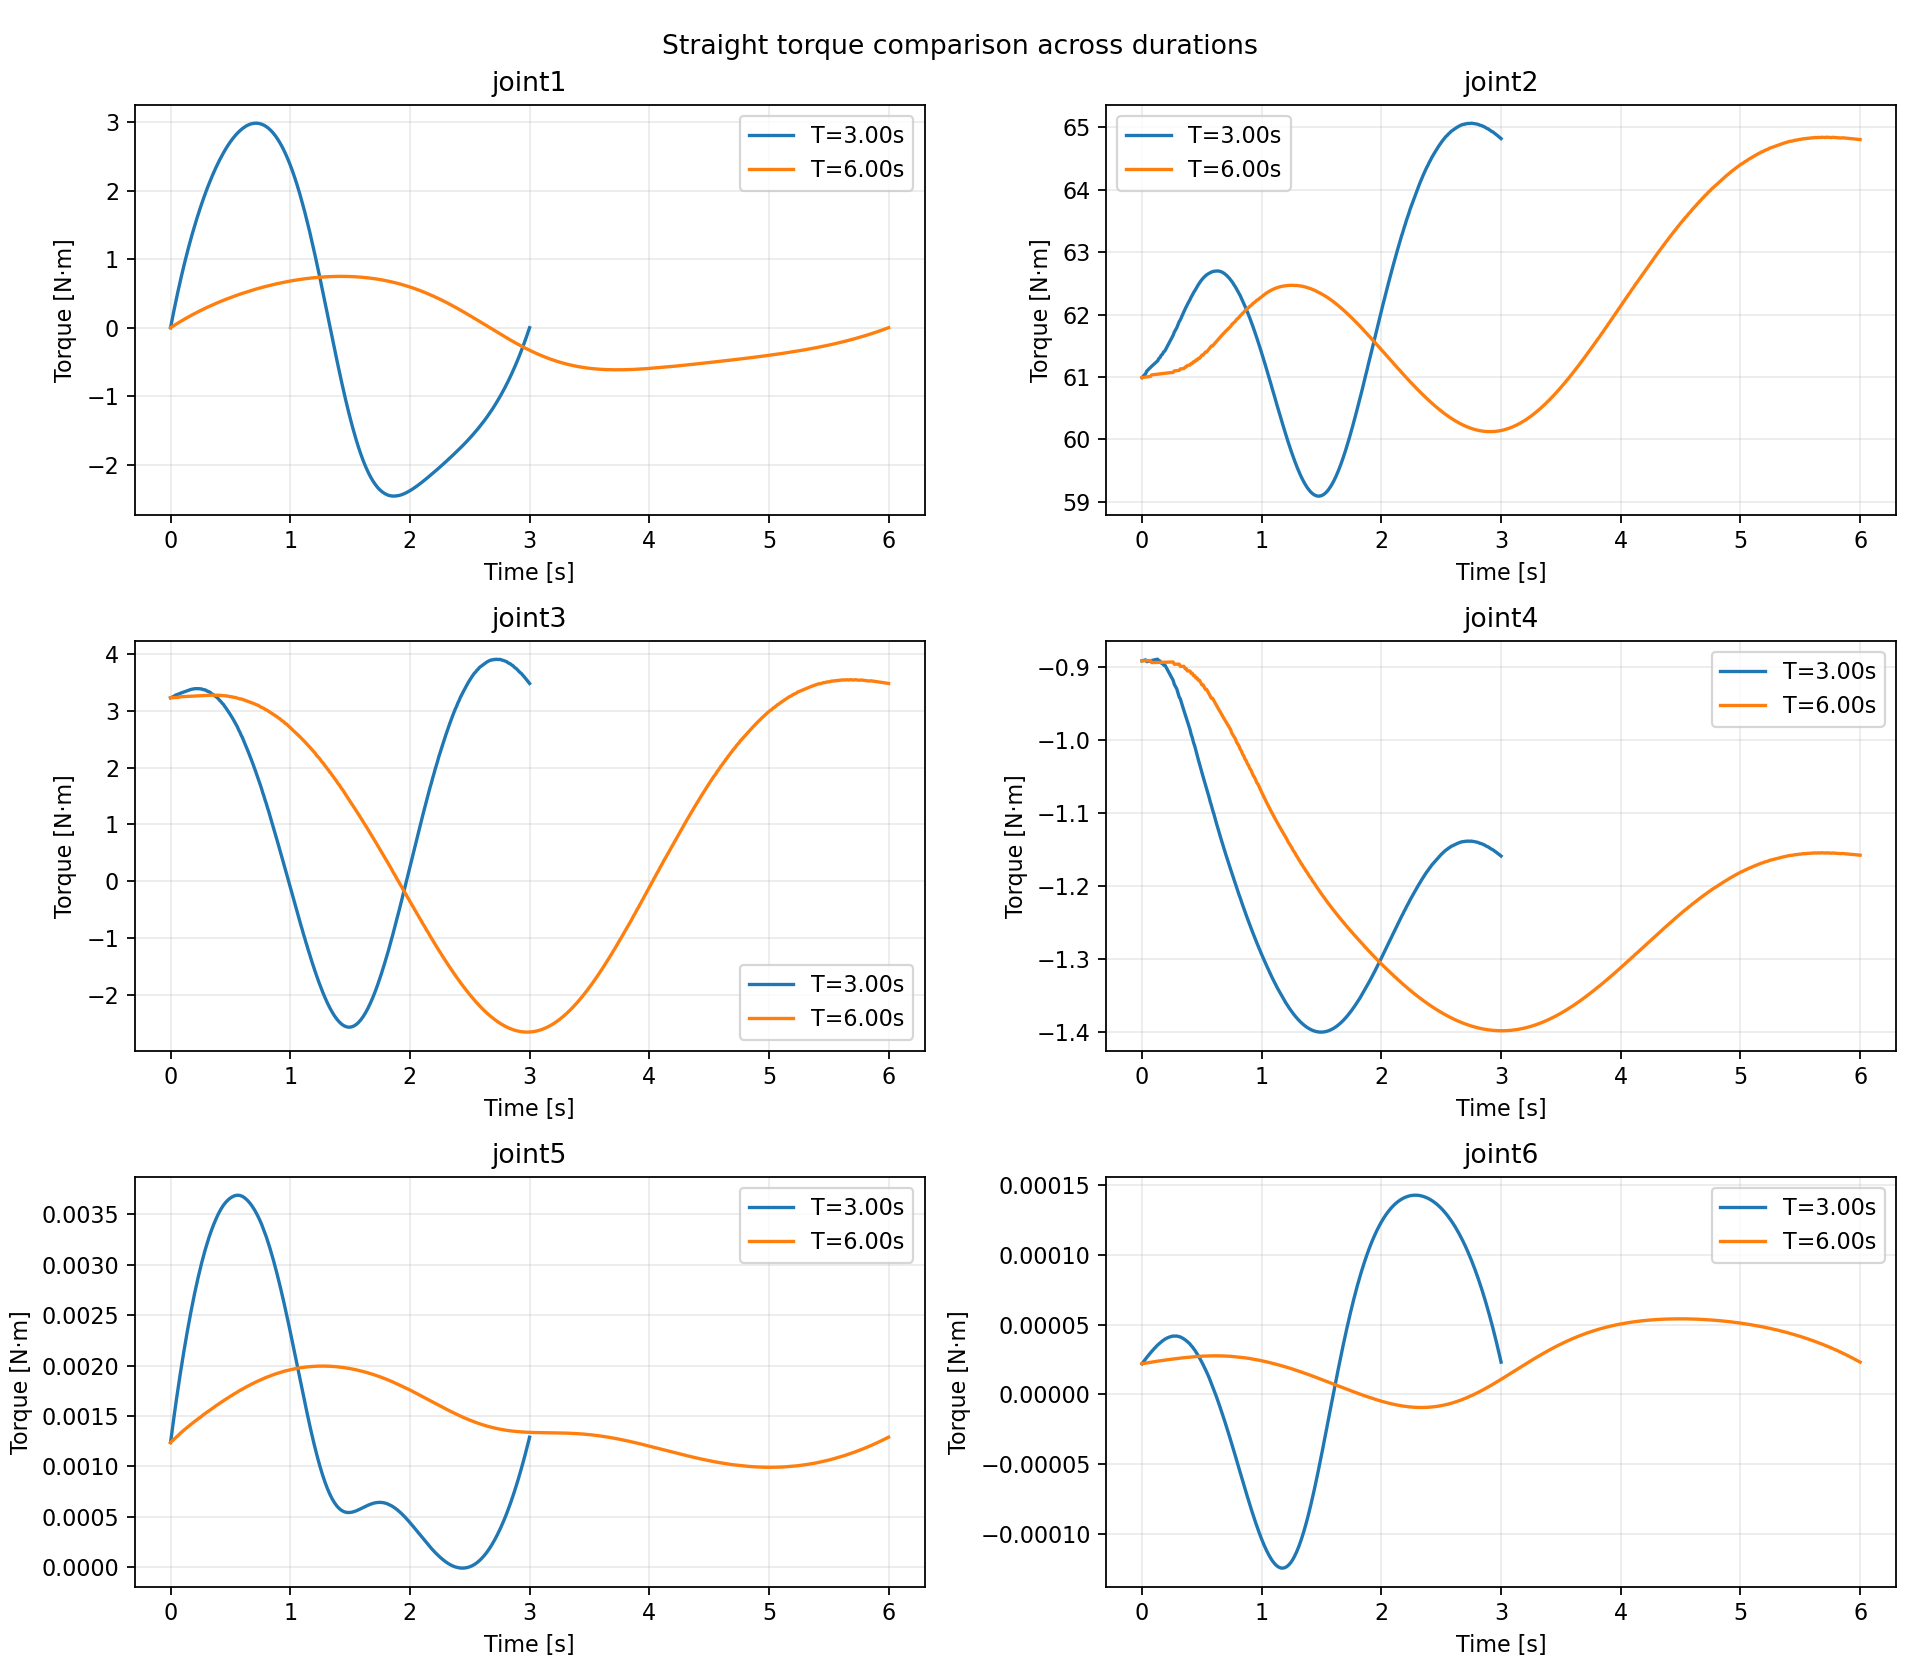
\includegraphics[width=1.0\textwidth]{straight_torque_duration_comparison.png}
    \caption{Straight-line trajectory: torque comparison for $T=\SI{3}{s}$ and $T=\SI{6}{s}$.}
    \label{fig:straight_duration_comparison}
\end{figure}

\begin{figure}[H]
    \centering
    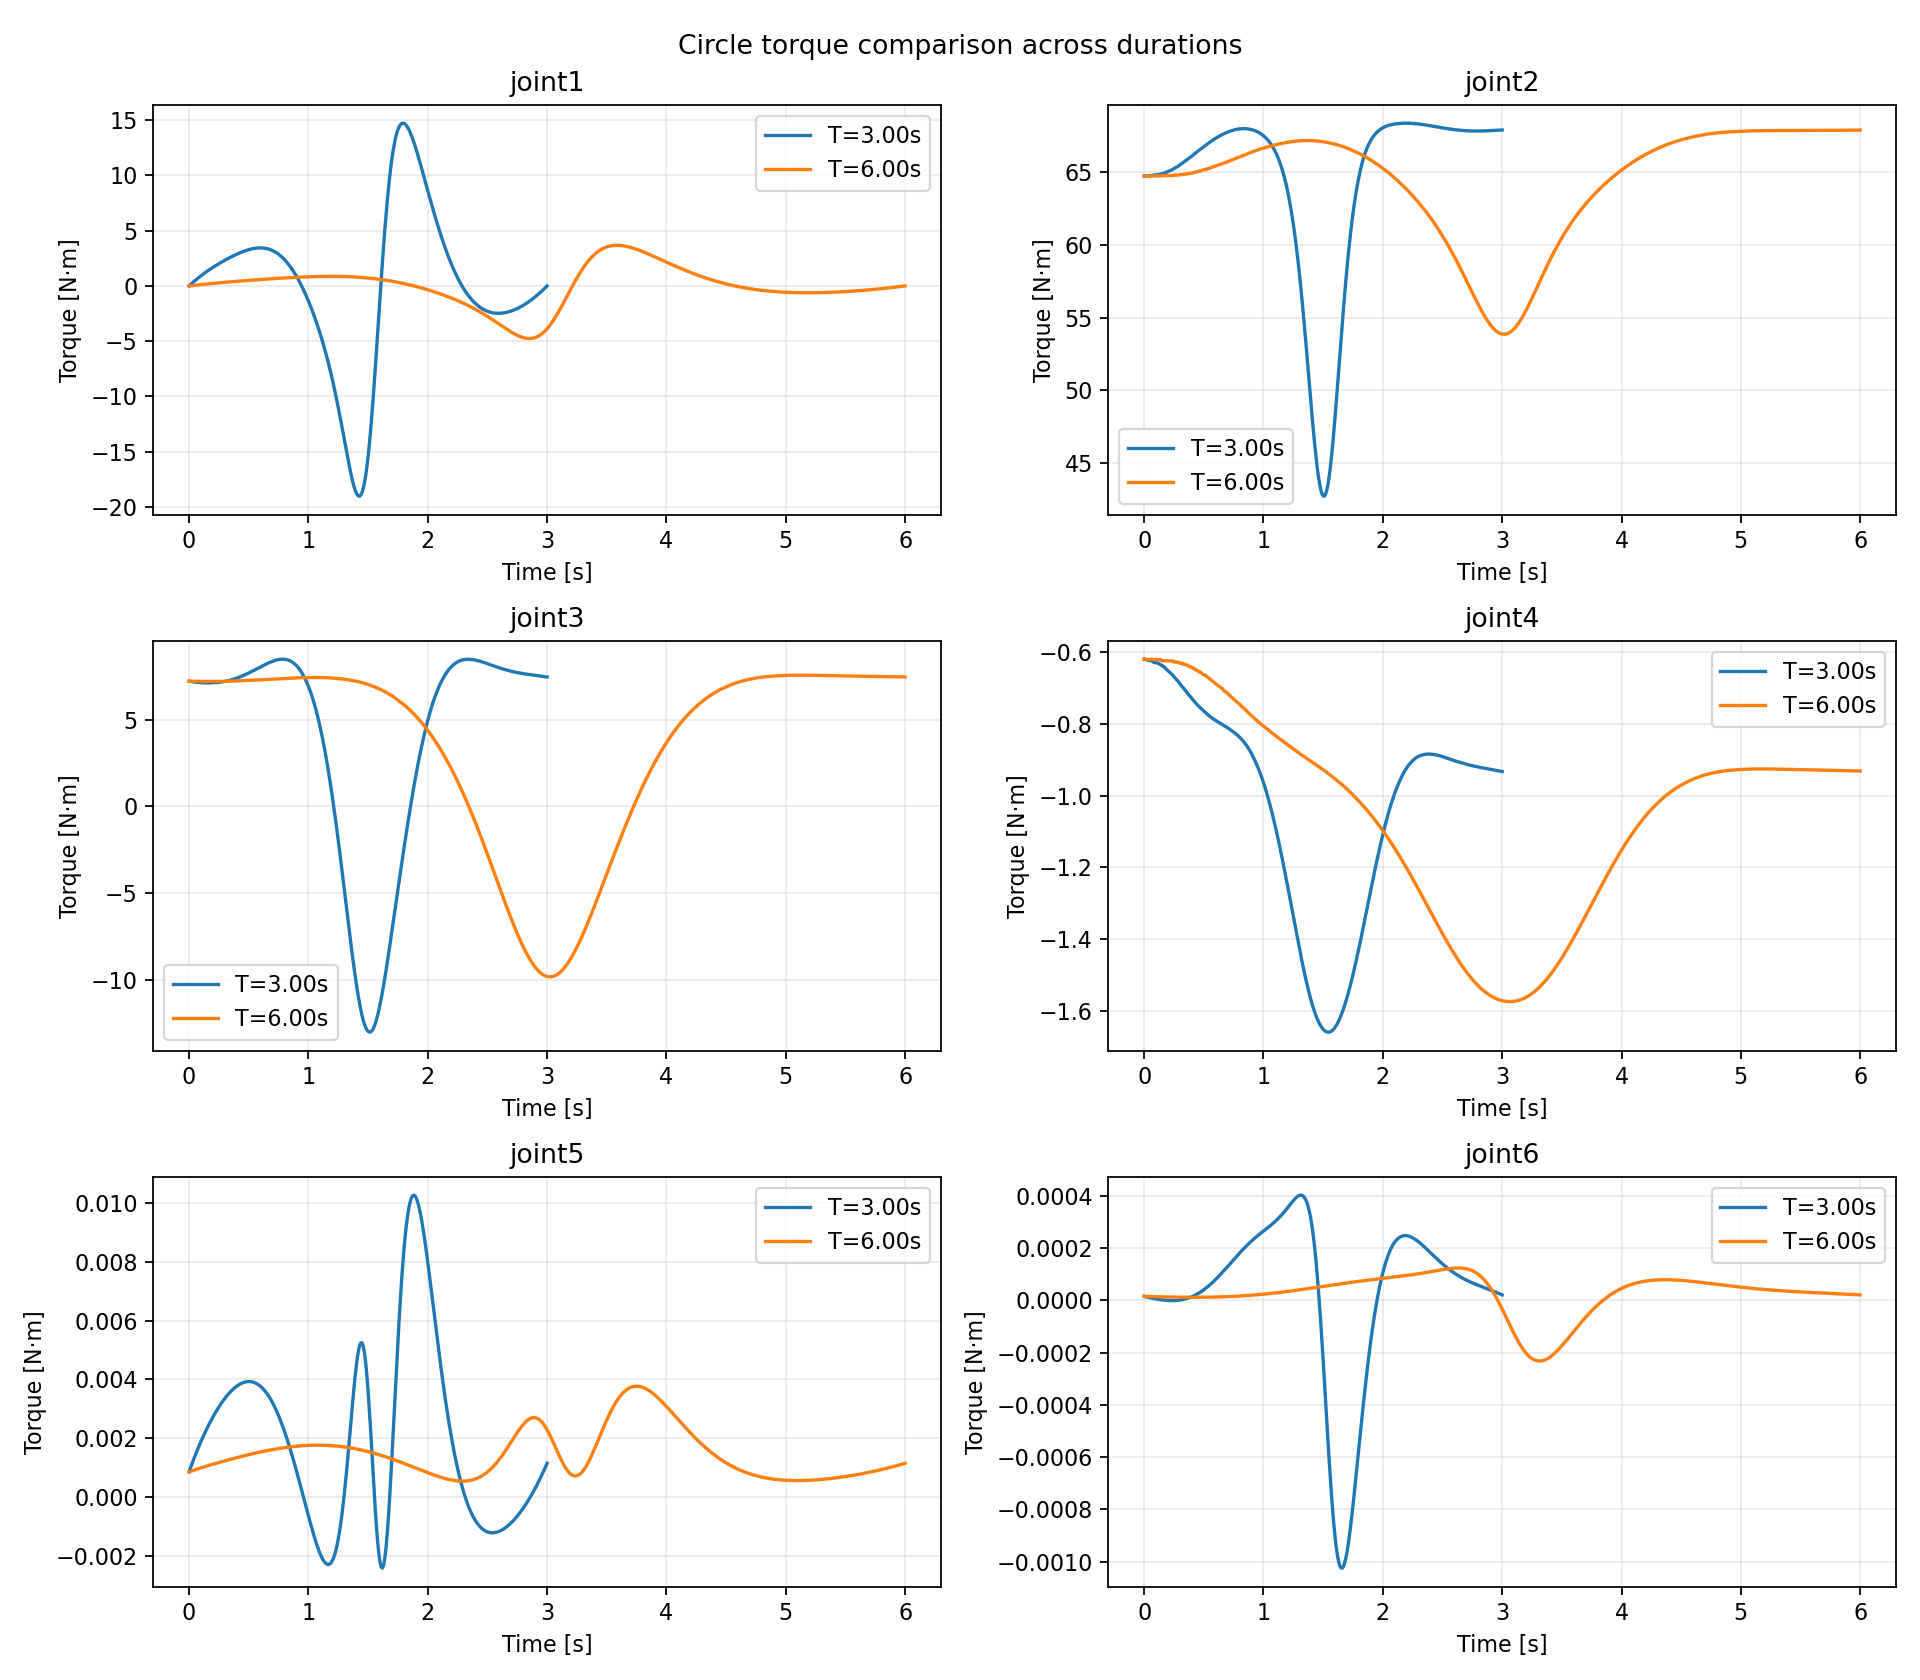
\includegraphics[width=1.0\textwidth]{circle_torque_duration_comparison.png}
    \caption{Circular trajectory: torque comparison for $T=\SI{3}{s}$ and $T=\SI{6}{s}$.}
    \label{fig:circle_duration_comparison}
\end{figure}

% ============================================================
\section{Conclusion}
% ============================================================

This project implemented a complete kinematic and dynamic computation pipeline for the Dobot
CR10 manipulator. Starting from a desired Cartesian path, the pipeline produces joint positions
through inverse kinematics, joint velocities and accelerations through Jacobian-based
differential kinematics, and actuator torques through Pinocchio's RNEA inverse dynamics
solver. Two trajectories --- straight-line and circular --- were evaluated for two motion
durations, $T=\SI{3}{s}$ and $T=\SI{6}{s}$.

Several design decisions were critical for the correctness of the results. Using Pinocchio as
the sole kinematic model eliminated the numerical inconsistency that would arise from mixing a
symbolic model in IK with the Pinocchio Jacobian in Part~B. Using a position-only IK task with
nullspace regularization (continuity, joint-centering, and a fixed joint-6 anchor) prevented
wrist winding while preserving smooth trajectory tracking. Merging the Jacobian and
Jacobian-derivative computations into a single time step ensured that $\dot{J}_p$ was always
evaluated at the same $(\bm{q}_k, \dot{\bm{q}}_k)$ pair used to compute $\ddot{\bm{q}}_k$.
The RNEA boundary check provided a physics-based consistency test that the computed torques
satisfy $\bm{\tau} = \bm{g}(\bm{q})$ at the zero-velocity, zero-acceleration endpoints of the
quintic profile.

The duration study confirmed the theoretical scaling behavior of time-scaled trajectories:
velocity peaks scale as $1/T$ and acceleration peaks scale as $1/T^2$ when the path geometry
is held constant. Maximum torque does not scale by the same factor because gravity loading
is configuration-dependent and independent of trajectory speed. Joint 2 set the maximum torque
envelope in all four runs, while joints 1 and 3 carried the next-largest dynamic peaks
depending on trajectory geometry. The circular trajectory was dynamically more demanding than
the straight-line
trajectory in velocity, acceleration, and torque peaks, principally because of the centripetal
acceleration term that has no counterpart in linear motion.

\end{document}
